%%
%% This is file `extended-abstract',
%% generated with the docstrip utility.
%%
%% The original source files were:
%%
%% samples.dtx  (with options: `all,journal,bibtex,acmtog')
%% 
%% IMPORTANT NOTICE:
%% 
%% For the copyright see the source file.
%% 
%% Any modified versions of this file must be renamed
%% with new filenames distinct from sample-acmtog.tex.
%% 
%% For distribution of the original source see the terms
%% for copying and modification in the file samples.dtx.
%% 
%% This generated file may be distributed as long as the
%% original source files, as listed above, are part of the
%% same distribution. (The sources need not necessarily be
%% in the same archive or directory.)
%%
%%
%% Commands for TeXCount
%TC:macro \cite [option:text,text]
%TC:macro \citep [option:text,text]
%TC:macro \citet [option:text,text]
%TC:envir table 0 1
%TC:envir table* 0 1
%TC:envir tabular [ignore] word
%TC:envir displaymath 0 word
%TC:envir math 0 word
%TC:envir comment 0 0
%%
%% The first command in your LaTeX source must be the \documentclass
%% command.
%%
%% For submission and review of your manuscript please change the
%% command to \documentclass[manuscript, screen, review]{acmart}.
%%
%% When submitting camera ready or to TAPS, please change the command
%% to \documentclass[sigconf]{acmart} or whichever template is required
%% for your publication.
%%
%%

\documentclass[sigconf,nonacm,natbib=true]{acmart}

%%
%% \BibTeX command to typeset BibTeX logo in the docs
\AtBeginDocument{%
  \providecommand\BibTeX{{%
    Bib\TeX}}}

%% Rights management information.  This information is sent to you
%% when you complete the rights form.  These commands have SAMPLE
%% values in them; it is your responsibility as an author to replace
%% the commands and values with those provided to you when you
%% complete the rights form.
\setcopyright{acmlicensed}
\copyrightyear{2018}
\acmYear{2018}
\acmDOI{XXXXXXX.XXXXXXX}

%%
%% These commands are for a JOURNAL article.
\acmJournal{TOG}
\acmVolume{37}
\acmNumber{4}
\acmArticle{111}
\acmMonth{8}

%%
%% Submission ID.
%% Use this when submitting an article to a sponsored event. You'll
%% receive a unique submission ID from the organizers
%% of the event, and this ID should be used as the parameter to this command.
%%\acmSubmissionID{123-A56-BU3}

%%
%% For managing citations, it is recommended to use bibliography
%% files in BibTeX format.
%%
%% You can then either use BibTeX with the ACM-Reference-Format style,
%% or BibLaTeX with the acmnumeric or acmauthoryear sytles, that include
%% support for advanced citation of software artefact from the
%% biblatex-software package, also separately available on CTAN.
%%
%% Look at the sample-*-biblatex.tex files for templates showcasing
%% the biblatex styles.
%%

%%
%% The majority of ACM publications use numbered citations and
%% references.  The command \citestyle{authoryear} switches to the
%% "author year" style.
%%
%% If you are preparing content for an event
%% sponsored by ACM SIGGRAPH, you must use the "author year" style of
%% citations and references.
% \citestyle{acmauthoryear}

\usepackage{anyfontsize}
\usepackage{listings}
\usepackage[nolist]{acronym}
\usepackage{cleveref}
\usepackage{url}
\usepackage{tikz}
\usepackage{enumitem}
\crefname{equation}{}{}
\Crefname{equation}{}{}
\usetikzlibrary{shapes.geometric, arrows.meta, positioning, fit}
% These packages are required for list code snippets.
\usepackage{xcolor}
\usepackage{color}
% The following special color definitions are used in the IST Thesis
\definecolor{forestgreen}{RGB}{34,139,34}
\definecolor{orangered}{RGB}{239,134,64}
\definecolor{lightred}{rgb}{1,0.4,0.5}
\definecolor{orange}{rgb}{1,0.45,0.13}
\definecolor{darkblue}{rgb}{0.0,0.0,0.6}
\definecolor{lightblue}{rgb}{0.1,0.57,0.7}
\definecolor{gray}{rgb}{0.4,0.4,0.4}
\definecolor{lightgray}{rgb}{0.95, 0.95, 0.95}
\definecolor{darkgray}{rgb}{0.4, 0.4, 0.4}
\definecolor{editorGray}{rgb}{0.95, 0.95, 0.95}
\definecolor{editorOcher}{rgb}{1, 0.5, 0} % #FF7F00 -> rgb(239, 169, 0)
\definecolor{chaptergrey}{rgb}{0.6,0.6,0.6}
\definecolor{editorGreen}{rgb}{0, 0.5, 0} % #007C00 -> rgb(0, 124, 0)
\definecolor{olive}{rgb}{0.17,0.59,0.20}
\definecolor{brown}{rgb}{0.69,0.31,0.31}
\definecolor{purple}{rgb}{0.38,0.18,0.81}

\newcommand{\changed}[1]{\textcolor{orange}{#1}}

% Symbols for linear logic
\usepackage{cmll}

% For proof trees
\usepackage{bussproofs}

% For multiply counters, which I use for indentation in class environments
\usepackage{calc}

% These are useful!
\providecommand\todo{}
\renewcommand{\todo}[1]{\textcolor{red}{\textbf{#1}}}

% Useful for CLASS snippets
\lstdefinelanguage{CLASS}{
    morekeywords={proc, cut, close, wait, case, of, send, recv, choice, offer, !, ?, print, println, par, let, share, put, take, cell},
    morekeywords=[2]{lint, colint, lbool, colbool, state, usage},
    sensitive=true,
    moredelim=[is][keywordstyle2]{@}{@},
}

% Useful for IR snippets
\lstdefinelanguage{IR}{
    morekeywords={int, bool, string, tag, cont, exponential, cell, type, isValue},
    morecomment=[l]{//},
    sensitive=true,
}

% Color BNF with strings
\lstdefinelanguage{BNF}{
    morekeywords={nl, pid, lab, int, loc, t, t1, t2, c, c1, c2, d, d1, d2, e, prog, proc, entry, block, instr, sl, st, sc, ofs, locb, reqs, flag, expr, tflg, targ, carg, darg, parg, pargs, earg, eargs, case, if, else, str, bool, src, dst},
    sensitive=true,
    morestring=[b]",
    morestring=[b]',
    morecomment=[l]{//},
    morecomment=[s]{/*}{*/},
    moredelim=[is][keywordstyle2]{@}{@},
    alsoletter={:},
    morekeywords=[2]{::=,|,*,+,?},
}

% Slot names
\newcommand{\irs}[1]{\text{\textcolor{lightblue}{#1}}}
\newcommand{\ints}{\irs{int}}
\newcommand{\bools}{\irs{bool}}
\newcommand{\strings}{\irs{string}}
\newcommand{\tags}{\irs{tag}}
\newcommand{\conts}{\irs{cont}}
\newcommand{\exponentials}{\irs{exponential}}
\newcommand{\types}{\irs{type}}
\newcommand{\cells}[1]{\irs{cell}\left[#1\right]}
\newcommand{\vars}[1]{t_{#1}}

% Slot trees
\newcommand{\nilst}{\left[\right]}
\newcommand{\seqst}[1]{\left[#1\right]}
\newcommand{\tagst}[1]{\irs{tag}\left[#1\right]}
\newcommand{\flagsst}[3]{\irs{flags}\left<#1\right>\left[#2\tagsepst{}#3\right]}
\newcommand{\combst}[1]{\text{$<$}#1\text{$>$}}
\newcommand{\tagsepst}{\text{ | }}
\newcommand{\concatst}[2]{#1\oplus#2}

% Slot offset and data location
\newcommand{\offs}[2]{#1\text{$\sim$}#2}
\newcommand{\dataol}[2]{#1.#2}
\newcommand{\datal}[3]{\dataol{#1}{\offs{#2}{#3}}}

% Some notation commands
\newcommand{\sizeof}[1]{\phi\bigl(#1\bigr)}
\newcommand{\dual}[1]{\overline{#1}}
\newcommand{\getinstructions}[3]{\mathcal{I}_P(#1,\,#2,\,#3)}
\newcommand{\getendpoints}[2]{\mathcal{E}(#1,\,#2)}
\newcommand{\getexpression}[2]{\mathcal{I}_E(#1,\,#2)}
\newcommand{\makeblock}[1]{#1 \leftarrow \text{new}_{\text{b}}()}
\newcommand{\makecont}[1]{#1 \leftarrow \text{new}_{\text{c}}()}
\newcommand{\makedata}[2]{#1 \leftarrow \text{new}_{\text{d}}(#2)}
\newcommand{\makedrop}[3]{#1 \leftarrow \text{new}_{\text{e}}(#2,\,#3)}

% Type names
\newcommand{\classt}[1]{\textbf{\textcolor{forestgreen}{#1}}}
\newcommand{\closet}{\classt{close}}
\newcommand{\waitt}{\classt{wait}}
\newcommand{\lintt}{\classt{lint}}
\newcommand{\colintt}{\classt{colint}}
\newcommand{\lboolt}{\classt{lbool}}
\newcommand{\colboolt}{\classt{colbool}}
\newcommand{\lstringt}{\classt{lstring}}
\newcommand{\colstringt}{\classt{colstring}}
\newcommand{\choicet}[1]{\classt{choice of}\,\{#1\}}
\newcommand{\offert}[1]{\classt{offer of}\,\{#1\}}
\newcommand{\labelt}[2]{\classt{$|$\##1}:#2}
\newcommand{\sendt}[2]{\classt{send}\,#1;#2}
\newcommand{\recvt}[2]{\classt{recv}\,#1;#2}
\newcommand{\bangt}[1]{\classt{!}#1}
\newcommand{\whynott}[1]{\classt{?}#1}
\newcommand{\sendtyt}[2]{\classt{sendty}\,#1;#2}
\newcommand{\recvtyt}[2]{\classt{recvty}\,#1;#2}
\newcommand{\statet}[1]{\classt{state}\,#1}
\newcommand{\statelt}[1]{\classt{statel}\,#1}
\newcommand{\usaget}[1]{\classt{usage}\,#1}
\newcommand{\usagelt}[1]{\classt{usagel}\,#1}
\newcommand{\affinet}[1]{\classt{affine}\,#1}
\newcommand{\coaffinet}[1]{\classt{coaffine}\,#1}
\newcommand{\dualt}[1]{\classt{$\sim$}#1}
\newcommand{\rect}[2]{\classt{rec}\ #1;\,#2}
\newcommand{\corect}[2]{\classt{corec}\ #1;\,#2}

% Process names
\newcommand{\classp}[1]{\textbf{\textcolor{darkblue}{#1}}}
\newcommand{\emptyp}{\classp{()}}
\newcommand{\fwdp}{\classp{fwd}}
\newcommand{\cutp}{\classp{cut}}
\newcommand{\parp}{\classp{par}}
\newcommand{\closep}{\classp{close}}
\newcommand{\waitp}{\classp{wait}}
\newcommand{\casep}{\classp{case of}}
\newcommand{\labelp}[1]{\classp{\##1}}
\newcommand{\sendp}{\classp{send}}
\newcommand{\recvp}{\classp{recv}}
\newcommand{\bangp}{\classp{!}}
\newcommand{\whynotp}{\classp{?}}
\newcommand{\callp}{\classp{call}}
\newcommand{\sendtyp}{\classp{sendty}}
\newcommand{\recvtyp}{\classp{recvty}}
\newcommand{\unfoldmup}{\classp{unfold$_\mu$}}
\newcommand{\unfoldnup}{\classp{unfold$_\nu$}}
\newcommand{\corecp}{\classp{corec}}
\newcommand{\sharep}{\classp{share}}
\newcommand{\affinep}{\classp{affine}}
\newcommand{\discardp}{\classp{discard}}
\newcommand{\usep}{\classp{use}}
\newcommand{\cellp}{\classp{cell}}
\newcommand{\releasep}{\classp{release}}
\newcommand{\takep}{\classp{take}}
\newcommand{\putp}{\classp{put}}
\newcommand{\ifp}{\classp{if}}
\newcommand{\elsep}{\classp{else}}
\newcommand{\letp}{\classp{let}}
\newcommand{\scanp}{\classp{scan}}
\newcommand{\printp}{\classp{print}}
\newcommand{\printlnp}{\classp{println}}

% CLASS
\newcommand{\fwdc}[2]{\fwdp\,#1\,#2}
\newcommand{\cutc}[3]{\cutp\,\{#1\,\classp{$|$}#2\classp{$|$}\,#3\}}
\newcommand{\parc}[2]{\parp\,\{#1\,\classp{$||$}\,#2\}}
\newcommand{\emptyc}{\emptyp}
\newcommand{\closec}[1]{\closep\,#1}
\newcommand{\waitc}[1]{\waitp\,#1;}
\newcommand{\choosec}[2]{\classp{\##1}\ #2;}
\newcommand{\casec}[2]{\classp{case}\,#1\,\classp{of}\,\{#2\}}
\newcommand{\labelc}[2]{\classp{$|$}\labelp{#1}:#2}
\newcommand{\sendc}[3]{\sendp\,#1(#2.\,#3);}
\newcommand{\recvc}[2]{\recvp\,#1(#2);}
\newcommand{\bangc}[2]{\bangp\,#1(#2);}
\newcommand{\whynotc}[1]{\whynotp\,#1;}
\newcommand{\callc}[2]{\callp\,#1(#2);}
\newcommand{\sendtyc}[2]{\sendtyp\,#1(#2);}
\newcommand{\recvtyc}[2]{\recvtyp\,#1(#2);}
\newcommand{\unfoldmuc}[1]{\unfoldmup\,#1;}
\newcommand{\unfoldnuc}[1]{\unfoldnup\,#1;}
\newcommand{\corecc}[4]{\corecp\,#1(#2);\,#3\ [#4]}
\newcommand{\typedefc}[2]{\classp{type}\ #1\,\{#2\};;}
\newcommand{\rectypedefc}[2]{\classp{rec}\ \typedefc{#1}{#2}}
\newcommand{\typedefgc}[3]{\classp{type}\ #1(#2)\,\{#3\};;}
\newcommand{\rectypedefgc}[3]{\classp{rec}\ \typedefgc{#1}{#2}{#3}}
\newcommand{\procdefc}[3]{\classp{proc}\ \texttt{#1}(#2)\,\{#3\};;}
\newcommand{\procdefgc}[4]{\classp{proc}\ \texttt{#1}\langle#2\rangle(#3)\,\{#4\};;}
\newcommand{\recprocdefc}[3]{\classp{rec}\ \procdefc{#1}{#2}{#3}}
\newcommand{\recprocdefgc}[4]{\classp{rec}\ \procdefgc{#1}{#2}{#3}{#4}}
\newcommand{\proccallc}[2]{\texttt{#1}(#2)}
\newcommand{\proccallgc}[3]{\texttt{#1}\langle#2\rangle(#3)}
\newcommand{\sharec}[3]{\sharep\,#1\,\{#2\,\classp{$||$}\,#3\}}
\newcommand{\affinec}[1]{\affinep\,#1;}
\newcommand{\discardc}[1]{\discardp\,#1}
\newcommand{\usec}[1]{\usep\,#1;}
\newcommand{\cellc}[3]{\cellp\,#1(#2.\,#3)}
\newcommand{\cellfc}[2]{\cellp\,#1(#2)}
\newcommand{\releasec}[1]{\releasep\,#1}
\newcommand{\takec}[2]{\takep\,#1(#2);}
\newcommand{\putc}[3]{\putp\,#1(#2.\,#3);}
\newcommand{\putfc}[2]{\putp\,#1(#2);}
\newcommand{\ifc}[3]{\ifp\,#1\,\{#2\}\,\elsep\,\{#3\}}
\newcommand{\letc}[2]{\letp\,#1\,#2}
\newcommand{\scanc}[1]{\scanp(#1)}
\newcommand{\printc}[1]{\printp(#1);}
\newcommand{\printlnc}[1]{\printlnp(#1);}

% IR Data Locations
\newcommand{\slotoffset}[2]{#1\text{$\sim$}#2}
\newcommand{\offsetpast}[1]{\text{past}(#1)}
\newcommand{\offsetfuture}[1]{\text{future}(#1)}

% CLASS definitions
\newcommand{\slots}[2]{\mathcal{S}(#1,\,#2)}
\newcommand{\allslots}[2]{\mathcal{S}_T(#1,\,#2)}
\newcommand{\alllocalslots}[2]{\mathcal{S}_L(#1,\,#2)}

% Compiler environment accessors
\newcommand{\polarityof}[2]{#1_{p}(#2)}
\newcommand{\typeidof}[2]{#1_{t}(#2)}
\newcommand{\continuationof}[2]{#1_c(#2)}
\newcommand{\localdataof}[2]{#1_d(#2)}
\newcommand{\offsetof}[2]{#1_o(#2)}
\newcommand{\readlocof}[2]{#1_r(#2)}
\newcommand{\writelocof}[2]{#1_w(#2)}
\newcommand{\advancech}[6]{#1[#2 \overset{#3,#4}{\oplus} (#5,\,#6)]}

% C generator notation
\newcommand{\arch}{\mathcal{T}}
\newcommand{\archlayout}[1]{\arch(\texttt{#1})}
\newcommand{\slotlayout}[2]{\mathcal{L}_{\arch}(#1,\,#2)}
\newcommand{\layoutofvar}[2]{#1(#2)}
\newcommand{\envlayout}{\mathcal{E}}
\newcommand{\envlayouteps}[1]{\envlayout_\text{eps}(#1)}
\newcommand{\envlayoutdrop}[1]{\envlayout_\text{e}(#1)}
\newcommand{\envlayouttype}[2]{\envlayout_\text{ty}(#1, #2)}
\newcommand{\envlayoutcont}[2]{\envlayout_\text{c}(#1, #2)}
\newcommand{\envlayoutlocal}[2]{\envlayout_\text{d}(#1, #2)}

% Optimizer notation
\newcommand{\typeenv}{\theta}
\newcommand{\isvalue}[1]{\mathcal{V}_\typeenv(#1)}
\newcommand{\isdroppable}[1]{\mathcal{D}_\typeenv(#1)}
\newcommand{\iscloneable}[1]{\mathcal{C}_\typeenv(#1)}
\newcommand{\impossible}{\mathbf{impossible}}
\newcommand{\guaranteed}{\mathbf{guaranteed}}
\newcommand{\dependent}[1]{\mathbf{dependent}(#1)}
\newcommand{\depisvalue}[1]{\mathcal{V}(#1)}
\newcommand{\depisdroppable}[1]{\mathcal{D}(#1)}
\newcommand{\depiscloneable}[1]{\mathcal{C}(#1)}

% Session modes
\newcommand{\writemode}{\texttt{write}}
\newcommand{\readmode}{\texttt{read}}

% Indented CLASS environment
\newcounter{indentlevel}
\newlength{\indentstep}
\newenvironment{class}
{
    \begingroup

    \setcounter{indentlevel}{0}

    \setlength{\indentstep}{1.5em}

    \newcommand{\iz}{\addtocounter{indentlevel}{1}}
    \newcommand{\dz}{\addtocounter{indentlevel}{-1}}
    \newcommand{\pz}{\hspace*{\the\indentstep*\value{indentlevel}}}
    \newcommand{\z}{\\&\pz}

    % CLASS
    \let\cuti\cutc
    \renewcommand{\cutc}[3]{\cuti{\iz\z##1\z}{##2}{\z##3\dz\z}}
    \let\pari\parc
    \renewcommand{\parc}[2]{\pari{\iz\z##1\z}{\z##2\dz\z}}
    \let\waiti\waitc
    \renewcommand{\waitc}[1]{\waiti{##1}\z}
    \let\sendi\sendc
    \renewcommand{\sendc}[3]{\sendi{##1}{##2}{##3}\z}
    \let\recvi\recvc
    \renewcommand{\recvc}[2]{\recvi{##1}{##2}\z}
    \let\choosei\choosec
    \renewcommand{\choosec}[2]{\choosei{##1}{##2}\z}
    \let\casei\casec
    \renewcommand{\casec}[2]{\casei{##1}{##2\z}}
    \let\labeli\labelc
    \renewcommand{\labelc}[2]{\iz\z\labeli{##1}{##2}\dz}
    \let\unfoldmui\unfoldmuc
    \renewcommand{\unfoldmuc}[1]{\unfoldmui{##1}\z}
    \let\unfoldnui\unfoldnuc
    \renewcommand{\unfoldnuc}[1]{\unfoldnui{##1}\z}
    \let\procdefi\procdefc
    \renewcommand{\procdefc}[3]{\procdefi{##1}{##2}{\iz\z##3\dz\z}}
    \let\procdefgi\procdefgc
    \renewcommand{\procdefgc}[4]{\procdefgi{##1}{##2}{##3}{\iz\z##4\dz\z}}
    \let\typedefi\typedefc
    \renewcommand{\typedefc}[2]{\typedefi{##1}{\iz\z##2\dz\z}}
    \let\typedefgi\typedefgc
    \renewcommand{\typedefgc}[3]{\typedefgi{##1}{##2}{\iz\z##3\dz\z}}
    \let\printi\printc
    \renewcommand{\printc}[1]{\printi{##1}\z}
    \let\printlni\printlnc
    \renewcommand{\printlnc}[1]{\printlni{##1}\z}
    \let\affinei\affinec
    \renewcommand{\affinec}[1]{\affinei{##1}\z}
    \let\usei\usec
    \renewcommand{\usec}[1]{\usei{##1}\z}
    \let\discardi\discardc
    \renewcommand{\discardc}[1]{\discardi{##1}}
    \let\celli\cellc
    \renewcommand{\cellc}[3]{\celli{##1}{##2}{\iz\z##3\dz\z}}
    \let\cellfi\cellfc
    \renewcommand{\cellfc}[2]{\cellfi{##1}{##2}\z}
    \let\takei\takec
    \renewcommand{\takec}[2]{\takei{##1}{##2}\z}
    \let\puti\putc
    \renewcommand{\putc}[3]{\puti{##1}{##2}{##3}\z}
    \let\putfi\putfc
    \renewcommand{\putfc}[2]{\putfi{##1}{##2}\z}
    \let\sharei\sharec
    \renewcommand{\sharec}[3]{\sharei{##1}{\iz\z##2\z}{\z##3\dz\z}}

    $$
        \begin{aligned}
             & \pz
            }
            {
        \end{aligned}
    $$

    \endgroup
}

% Compilation environment
\newenvironment{compilation}[4]
{
    \begingroup
    % IR
    \newcommand{\beginir}{\\&\hspace{2.5em}}
    \newcommand{\mkzeroargir}[2]{\newcommand{##1}{\beginir\texttt{##2}()}}
    \newcommand{\mkoneargir}[2]{\newcommand{##1}[1]{\beginir\texttt{##2}(####1)}}
    \newcommand{\mktwoargir}[2]{\newcommand{##1}[2]{\beginir\texttt{##2}(####1, ####2)}}
    \newcommand{\mkthreeargir}[2]{\newcommand{##1}[3]{\beginir\texttt{##2}(####1, ####2, ####3)}}
    \newcommand{\mkfourargir}[2]{\newcommand{##1}[4]{\beginir\texttt{##2}(####1, ####2, ####3, ####4)}}
    \newcommand{\labelir}[1]{\\&\hspace{1.25em}\texttt{##1:}}
    \renewcommand{\comment}[1]{\quad\textcolor{forestgreen}{\%\ ##1}}
    \newcommand{\commentline}[1]{\beginir\textcolor{forestgreen}{\%\ ##1}}

    \mkoneargir{\launchthread}{launchThread}
    \mkoneargir{\pushtask}{pushTask}
    \mkoneargir{\poptask}{popTask}
    \mktwoargir{\finishcont}{finish}
    \mkoneargir{\continue}{continue}
    \mkthreeargir{\bindcontinuation}{bindContinuation}
    \mkthreeargir{\forward}{forward}
    \mktwoargir{\branchtag}{branchTag}
    \mktwoargir{\branchflags}{branchFlags}
    \mktwoargir{\writetype}{writeType}
    \mktwoargir{\writetag}{writeTag}
    \mktwoargir{\writeexpr}{writeExpression}
    \mktwoargir{\writescan}{writeScan}
    \mktwoargir{\writecell}{writeCell}
    \mkthreeargir{\writeexp}{writeExponential}
    \mktwoargir{\writecontinuation}{writeContinuation}
    \mkoneargir{\lockcell}{lockCell}
    \mkoneargir{\unlockcell}{unlockCell}
    \mkoneargir{\acquirecell}{acquireCell}
    \mkoneargir{\releasecell}{releaseCell}
    \mkoneargir{\print}{print}
    \mkoneargir{\printline}{printLine}
    \mkfourargir{\continueifneg}{continueIfNegative}
    \mkthreeargir{\moveslots}{moveSlots}
    \mkthreeargir{\cloneslots}{cloneSlots}
    \mktwoargir{\dropslots}{dropSlots}
    \mkthreeargir{\callprocess}{callProcess}
    \mkoneargir{\deferdrop}{deferDrop}

    \mkoneargir{\newtask}{newTask}
    \mkzeroargir{\nexttask}{nextTask}
    \mkthreeargir{\initcontinuation}{initializeContinuation}
    \mkoneargir{\freesession}{freeSession}
    \mkthreeargir{\call}{call}
    \mkoneargir{\flip}{flip}
    \mktwoargir{\fwd}{fwd}
    \mkoneargir{\pushclose}{pushClose}
    \mkoneargir{\popclose}{popClose}
    \mktwoargir{\pushtag}{pushTag}
    \mktwoargir{\poptag}{popTag}
    \mktwoargir{\pushsession}{pushSession}
    \mktwoargir{\popsession}{popSession}
    \newcommand{\hasexitpoint}{\texttt{exit point}}
    \newcommand{\recurse}[3]{\beginir\getinstructions{##1}{##2}{##3}}

    $$
        \begin{aligned}
             & \getendpoints{#1}{#3} \equiv #4 \\
             & \getinstructions{#1}{#2}{#3} \equiv
            }
            {
        \end{aligned}
    $$
    \endgroup
}

% For \Mapsto
\usepackage{stmaryrd}

% For centering tables
\usepackage{tabularx}


\setlength{\abovecaptionskip}{0pt}
\setlength{\belowcaptionskip}{-10pt}

\lstset{
  basicstyle=\linespread{0.9}\ttfamily\small, % smaller and tighter
  columns=fixed,                              % prevents extra letter spacing
  frame=lines,                               % simple frame around code
  numbers=left,                               % line numbers on the left
  numberstyle=\tiny,                          % small line numbers
  stepnumber=1,                               % number every line
  numbersep=5pt,                              % space between numbers and code
  backgroundcolor=\color{white},              % optional: light background
  keywordstyle=[1]\color{darkblue}\bfseries,         % color keywords
  keywordstyle=[2]\color{forestgreen}\bfseries,       % color keywords
  commentstyle=\color{gray}\itshape,          % color comments
  stringstyle=\color{orange},                 % color strings
  showstringspaces=false                      % no visible spaces
}


\tikzset{
    frame/.style={draw, thick, fill=gray!10, inner sep=0pt},
    row/.style={
        fill=white,
        minimum width=6cm,
        minimum height=0.5cm,
        anchor=west,
        font=\ttfamily\small,
        inner xsep=6pt,
        text width=5.7cm,
        align=left,
        append after command={
            \pgfextra{\draw (\tikzlastnode.north west) -- (\tikzlastnode.north east);}
        }
    },
    arrow/.style={->, thick, >=Stealth},
    biarrow/.style={<->, thick, >=Stealth},
    doublearrow/.style={
        ->,
        double,
        line width=0.6pt,
        double distance=1pt,
        >=Stealth,
        thick
    }
}

\begin{acronym}
	\acro{IR}{Intermediate Representation}
	\acro{CLASS}{Classic Linear Logic with Affine Shared State}
	\acro{SAM}{Linear Session Abstract Machine}
	\acro{GCC}{GNU Compiler Collection}
	\acro{AST}{Abstract Syntax Tree}
	\acro{RSS}{Resident Set Size}
	\acro{FFI}{Foreign Function Interface}
	\acro{CCS}{Calculus of Communicating Systems}
	\acro{IST}{Instituto Superior Tecnico}
\end{acronym}

%%
%% end of the preamble, start of the body of the document source.
\begin{document}
\settopmatter{printfolios=true}

%%
%% The "title" command has an optional parameter,
%% allowing the author to define a "short title" to be used in page headers.
\title{Efficient Compilation for the Linear Language CLASS}

%%
%% The "author" command and its associated commands are used to define
%% the authors and their affiliations.
%% Of note is the shared affiliation of the first two authors, and the
%% "authornote" and "authornotemark" commands
%% used to denote shared contribution to the research.
\author{Ricardo Gomes de Oliveira Caeiro Antunes}
\affiliation{%
  \institution{Instituto Superior Técnico}
  \city{Lisboa}
  \country{Portugal}}
\email{me@riscadoa.com}
\authornote{Supervised by Prof. Luís Caires}

%%
%% By default, the full list of authors will be used in the page
%% headers. Often, this list is too long, and will overlap
%% other information printed in the page headers. This command allows
%% the author to define a more concise list
%% of authors' names for this purpose.
\renewcommand{\shortauthors}{Ricardo Antunes}

%%
%% The abstract is a short summary of the work to be presented in the
%% article.
\begin{abstract}
In this thesis we provide a comprehensive study of compilation techniques for high-level linear-typed (multiparadigm) languages, focusing on \ac{CLASS}, a proof-of-concept general purpose programming language based on linear/session types that supports many realistic concurrent programming idioms, while guaranteeing memory safety and  absence of deadlocks by typing.
While the principles and meta-theory behind linear logic based session languages are well known, associated implementation techniques for such languages, in particular compilation to native code, are still poorly understood. In this work, we leverage the sequential execution strategy of the \ac{SAM} to propose a novel multi-stage compilation scheme from CLASS to IR to C for a specially designed intermediate language IR,
implement a prototype compiler based on it, and validate it in terms of coverage, correctness and performance. Moreover, the developed compiler covers all of CLASS linear logic primitives, including affine sessions and shared state.  The performance of the compiled programs is compared with the original CLASS interpreter, the SAM interpreter, and with equivalent programs written in Haskell. The results show that the compiled programs are orders of magnitude faster than the interpreted ones, and, in some cases, outperform equivalent Haskell programs compiled with GHC. To the best of our knowledge this is the first work demonstrating the efficient compilation of linear session basic languages to machine code.
\end{abstract}

%%
%% Keywords. The author(s) should pick words that accurately describe
%% the work being presented. Separate the keywords with commas.
\keywords{Session types, Linear Logic, Compilation scheme, Intermediate representation, CLASS, Linear Session Abstract Machine (SAM)}

%%
%% This command processes the author and affiliation and title
%% information and builds the first part of the formatted document.
\maketitle

\section{Introduction}

\subsection{Motivation and Contributions}

Type systems are a powerful tool which can be used to ensure the absence of some runtime errors, which would otherwise require extensive testing or program analysis. Essentially, type systems form a set of rules which limit the programs that can be written in a given language. Most traditional compiled imperative languages, such as C and Java, have type systems that avoid some common programming errors, such as passing a string to a function that expects an integer. Although programs in a weakly or dynamically typed language such as Python or JavaScript would compile and run, they would likely fail at runtime, whereas in a strongly typed language, the compiler would catch the error at compile time. Strongly typed languages can additionally make use of their types to provide more information about the behavior of the code to the compiler, opening up new optimization paths.

More recently, substructural types have been proposed to statically ensure even stronger properties of the code, namely resource-usage properties related to memory manipulation, and protocol compliance, namely via linear types and session types~\citep{Wadler:1990,Honda:1998,Mostrous:2014}. In fact, linear and affine types are becoming more and more relevant in practice, as witnessed by the adoption of programming languages such as Rust \citep{Matsakis:2014}, for general systems programming, Move \citep{Move:2019, Move:2020}, for smart contracts, Linear Haskell \citep{Bernardy:2017}, and others \citep{Rast:2022, Ferrite:2022, C0:2016, FreeST:2019, Jacobs:2023} for general purpose programming. Session types have been used to enforce correctness in communication protocols, namely in languages based on process calculus, which model concurrent systems \citep{Milner:1980,Milner:1992:1,Milner:1992:2}. By coupling session types with linear logic \citep{Girard:1987,Caires:2010}, it has been possible to additionally guarantee deadlock freedom. 

\acs{CLASS} \citep{Rocha:2021, Rocha:2023, Rocha:2022} is a proof-of-concept general purpose linear programming language based on linear/session types.
\acs{CLASS} supports many realistic concurrent programming idioms, and is the first language to simultaneously guarantee memory safety and the absence of dead-locks.
%
However, the \acs{CLASS} interpreter implemented by \citet{Rocha:2021:artifact,Rocha:2023:artifact} served as a proof-of-concept for the language, and was not at all optimized for performance, and thus, wasn't suitable for real-world applications --- such fully concurrent implementations spawn threads for all concurrent processes, based on the ``default'' concurrent interpretation of session-based programs (e.g., ~\citep{FreeST:2019,Jespersen:2015}).
%

%
As a first step, the \acf{SAM}  was introduced by \citet{Caires:2024} to provide a formal model for sequentially executing the processes of session-typed languages, allowing for orders of magnitude better runtime performance.
However, although the \ac{SAM} design opens the way for the mechanical sequential execution of CLASS programs, it is still a formal abstract machine model, in the spirit of \citep{Landin:1964,Lafont:1988}. Therefore, the prototype implementation of the SAM \citep{Caires:2024:artifact} was of course expected to still introduce a heavy performance overhead, compared to a potential, still to be developed, version of the language implementation based on compilation to native code.

During this work, a compilation scheme was designed and implemented which translates \acs{CLASS} programs into efficient C code, while maintaining all of the safety and liveness guarantees of \acs{CLASS}. This approach allows a two orders of magnitude more efficient execution of \acs{CLASS} programs than the \ac{SAM} interpreter, as the compiler can make use of the extensive knowledge of the compiled programs. In some cases, the compiler even outperforms equivalent Haskell programs compiled with GHC. Moreover, the developed compiler supports all of \acs{CLASS}, including affine sessions and shared state.

\subsection{Compilation Overview}

\ac{CLASS} programs are linearly typed session-based programs. Programs are constructed by composing processes which communicate through channels. Channels are first-class citizens of the language, replacing variables from traditional imperative languages. Communication through channels is regulated by the channel's session type, which describes the communication protocol followed by the channel. The linearity of the type system ensures that all communication is carried out exactly once, preventing leakage of resources, and guaranteeing memory safety. An example \ac{CLASS} program is shown below.

\begin{lstlisting}[language=CLASS]
proc main() {
  cut {
    let x 1
    |x: colint|
    print(x); ()
  }
};;
\end{lstlisting}

This program defines a process \texttt{main} which will be executed when the program is run. Within it, the $\cutp$ process creates a new session $x$ through which both sides of the cut can communicate. On the right hand side of the cut, $x$ is typed by $\colintt$, and on the left hand side of the cut, by its dual, $\lintt$. Semantically, the left hand side of the cut must produce an integer, which the right hand side must then consume. In this case, the left hand side produces the integer 1, through the $\letp$ process, and the right hand side consumes it by printing it to the standard output, through the $\printp$ process. The $\printp$ process requires a continuation, which in this case is the $\emptyp$ process, which represents end of computation.

An \acf{IR} was developed to serve as an intermediate step between \ac{CLASS} and C code, greatly simplifying the compilation process. This \ac{IR} is based on the \ac{SAM} execution model, sequentially executing the processes of the \ac{CLASS} program with buffered communication. The final compilation scheme is divided into three main phases: the translation from \ac{CLASS} to \ac{IR}, optimization of the \ac{IR}, and generation of C code from the optimized \ac{IR}. The \ac{IR} translation of the previous example is shown below.
\begin{lstlisting}[language=IR]
main:
  exit points: 2
  continuations: c0
  data d0: <[int]> (c0)
entry:
  initializeContinuation(c0, cut_0, d0)
  writeExpression(c0, 1)
  finishContinuation(c0, exit point)
cut_0:
  print(move(d0, int))
  popTask(exit point)
\end{lstlisting}
Process $\texttt{main}$ is translated into an \ac{IR} process of the same name, composed of an header and a set of instruction blocks. The header specifies that the process has two exit points, a continuation $c_0$, used to implement session $x$, and a data section $d_0$, which will store the integer written to $x$.

The \texttt{entry} block of the \ac{IR} process is generated from the $\cutp$ process. It starts by initializing $c_0$, indicating its writing location to be $d_0$, and setting its return address to block \texttt{cut\_0}. The writing side is always executed first, so the next instructions are generated from the $\letp$ process. A write of the integer $1$ to the continuation $c_0$ (and thus to $d_0$) is generated, along with a \texttt{finishContinuation} instruction, which passes control to the return address \texttt{cut\_0} of $c_0$. The \texttt{cut\_0} block is generated from the right hand side of the cut. $\printp$ is translated to a \texttt{print} instruction, which reads the integer from $d_0$ and prints it. Finally, $\emptyp$ is translated to \texttt{popTask}, which, in this case, ends the program.

A set of transformations are applied to the \ac{IR} program to improve its performance, producing the final version of the \ac{IR}, shown below.
\begin{lstlisting}[language=IR]
main:
  exit points: 1
  data d0: <[int]>
entry:
  writeExpression(d0, 1)
  print(move(d0, int))
  popTask(exit point)
\end{lstlisting}
Using information obtained from a symbolic execution of the \ac{IR} program, the continuation $c_0$ can be optimized away entirely, leaving only the data variable $d_0$. In this case, since \texttt{finishSession} must pass control to the \texttt{cut\_0} block, it could be removed and the blocks concatenated. Furthermore, the writing location of $c_0$ is known to be $d_0$. Thus \texttt{writeExpression} can write directly to it.

Finally, the optimized \ac{IR} program is translated to C code. Due to the continuation-based nature of the \ac{SAM} execution model, processes are not represented as functions, but instead as code blocks within a single function, with control being transferred between them through the use of \texttt{goto} statements. Stack frames are replaced by heap-allocated environments, linked together to form a spaghetti stack. These environments contain all local variables and state used by the process. A set of variables are used as registers to keep the current execution state, such as a pointer \texttt{env} to the active environment. A segment of the generated code is shown below.
\begin{lstlisting}[language=C]
main_entry:
  *(int*)(env + 0) = 1;
  printf("%d", *(int*)(env + 0));
  managed_free(env);
\end{lstlisting}
The \texttt{main\_entry} label represents the \texttt{entry} block of the \ac{IR} \texttt{main} process. At the start of the program, an environment \texttt{env} is allocated and control is passed to this label. The \texttt{writeExpression} instruction is compiled into a simple assignment to the location of $d_0$ in the environment, which in this case is at offset $0$. The \texttt{print} instruction is compiled into a call to the C \texttt{printf} function, reading the integer from the same location. Finally, the \texttt{popTask} instruction is compiled into code which frees the current environment, and, in this case, ends the program.

\subsection{Document Structure}

The second section of this document provides the main background information required to understand the rest of the document, introducing the foundations of linear/session types, the \ac{CLASS} language and the Linear \ac{SAM}. The third section gives an overview of the compilation scheme, describing the compilation pipeline. The fourth section highlights the main developed optimizations. The fifth section briefly presents and discusses the obtained results. Finally, the sixth section concludes the document and suggests future work.

\section{Background and Related Work}

\subsection{Foundations of Linear Session Types}

\subsubsection{Process Calculi}

Multiple paradigms have been developed to model concurrent systems. One of the most well-known is \acf{CCS} \citep{Milner:1980}, which introduced the notion of parallel composition, restriction and communication. In the 90s, \citet{Milner:1992:1,Milner:1992:2} introduced $\pi$-calculus, a process calculus that allows for mobility of processes --- channels, through which processes communicate, can themselves be sent and received. It unifies data with communication channels, treating them as first-class citizens. This allows for more complex communication patterns, where the topology of the network can change dynamically. $\pi$-calculus can be used to encode various computation paradigms, such as $\lambda$-calculus and Turing machines, and thus, is a universal model of computation.

% Processes can be seen as a generalization of functions, where the input and output can be sent over a channel - a function call can be seen as sending the input over a channel, and then receiving the output over the same channel. Additionally, coroutine constructs and generator expressions common in modern languages such as Python can also be easily modeled as a process calculus, where calls to \textit{yield} statements can be seen as sending values over a channel. Channels in $\pi$-calculus can also be replicated, which makes it possible to model services that can be accessed by multiple clients, such as web servers.

\subsubsection{Linear Logic}

Introduced by \citet{Girard:1987}, linear logic is a logic where propositions are consumed exactly once, as opposed to classical logic where propositions can be used any number of times. This property makes linear logic ideal for modeling resources on real-world systems, opening pathways for multiple optimizations, such as in-place updates in functional languages \citep{Hofmann:2000}. Since its inception, linear logic has been seen as a good candidate for modeling the foundations of concurrent stateful systems \citep{Wadler:1990}. In fact, through the works of \citet{Abramsky:1993}, it has been found that classical linear logic can be interpreted computationally, and since then, this connection has been developed further by multiple authors \citep{Turner:1999}. More importantly for this work, the propositions-as-types correspondence of linear logic has proven useful for modeling concurrent systems \cite{Caires:2010}.

\subsubsection{Session Types}

Introduced by \citet{Honda:1993}, and expanded upon by \citet{Honda:1998}, session types are a type discipline for communication-based programming that ensures that the communication between two parties is well-typed. Essentially, session types are a type discipline for process calculi, where operations on channels obey the protocol defined by the session type. While in typed $\lambda$-calculus types are associated with terms, which denote functions and values, session types are associated with channels.

Operations on session types include sending and receiving, selection and branching, and recursion. Session types have been used to model and verify communication protocols, enforcing their correctness \citep{Huttel:2016}. They have been implemented in various programming languages, either as a language feature, such as in Scribble \citep{Yoshida:2014} and Effpi \citep{Scalas:2019}, or as a library, such as in Rust \citep{Jespersen:2015} and Haskell \citep{Pucella:2008}.

More recently, a direct correspondence between session types and linear logic has been established \citep{Caires:2010, Wadler:2012, Caires:2012, Caires:2016, Giunti:2016}, where session types can be interpreted as linear propositions, and vice-versa. Linear logic connectives are enough to describe the communication patterns of finite sessions.

\subsection{The CLASS Language}

\acf{CLASS} is an experimental language for session-based programs \citep{Rocha:2023, Rocha:2022, Rocha:2021}. It expands on the correspondence between session types and linear logic, adding affine types and shared state. Well-typed \ac{CLASS} programs, while still allowing for higher-order polymorphic functional code and even recursion, always terminate, never deadlock on communication or reference cell acquisition, and never leak memory.

As usual in session based programming languages, in \ac{CLASS} processes communicate through sessions. Each session has two endpoints (also referred to as channels), and each endpoint is associated with a session type, which describes the communication protocol that the endpoint must follow. $x: A$ denotes that the channel $x$ obeys type $A$. These types describe the direction, order and content of the messages exchanged. For example
\[
    x : \recvt{\dualt{\lintt}}{\sendt{\lboolt}{\closet}}
\]
describes a channel $x$ which receives an integer, then sends a boolean, and finally, is closed, after which communication stops. The dual connective $\dualt{A}$ represents the dual of type $A$, describing the type of the other endpoint of the session. For example, $y: \dualt{A}$
\[
    y : \sendt{\lintt}{\recvt{\dualt{\lboolt}}{\waitt}}
\]
would describe the other endpoint of $x$. $y$ sends an integer, then receives a boolean, and finally waits to be closed.

Session types can be seen as dynamic entities which evolve as the communication progresses. For example, $y$ would then become
\[
    y : \recvt{\dualt{\lboolt}}{\waitt}
\]

The most fundamental process composition operation in \ac{CLASS} is the $\cutp$ operator
\[
    \cutc{P}{x: A}{Q}
\]
which composes two processes $P$ and $Q$ that run concurrently and communicate through a session $x$, where the endpoint $x$ in $Q$ obeys type $A$, and the endpoint $x$ in $P$ obeys type $\dualt{A}$. This composition corresponds to the linear logic cut rule: no linear name other than $x$ appears simultaneously in both $P$ and $Q$. It restricts interactions between $P$ and $Q$ to the session $x$, which is essential to achieve desirable metatheoretical properties such as deadlock freedom.

Parallel composition of processes is expressed by the process
$$
    \parc{P}{Q}
$$
which runs $P$ and $Q$ concurrently, without any communication between them. This composition corresponds to the mix rule of linear logic: no linear name appears in both $P$ and $Q$.

For each session type, there is a corresponding action process which performs the action described by the type. For example, $\closec{x}$ closes a channel $x: \closet$, and the process $\sendc{x}{y}{P}{Q}$ sends a new channel $y: A$ through a channel $x: \sendt{A}{B}$.

A \ac{CLASS} program is composed of a collection of type and process definitions. A type definition associates a name to a session type $A$, and a process definition associates a name to a process $P$, which may be parametrized by type parameters and channel arguments.

The following example program defines the process \texttt{main}. On one side of the cut, a session $y$ is sent to $x$, implemented by $\letc{y}{1}$. On the receiving side, $y$ is received and bound to $z$. The integer received from $z$ is doubled and sent through $x$, which is then printed by the receiver. The program terminates on $\emptyp$.

\begin{lstlisting}[language=CLASS]
proc main() {
  cut {
    recv x(z); let x z * 2
    |x: @send@ lint; colint|
    send x(y. let y 1);
    println(x); ()
  }
};;
\end{lstlisting}

\subsection{The Linear Session Abstract Machine (SAM)}

The \ac{SAM}, introduced by \citet{Caires:2024}, is a virtual machine for executing session processes typed by (classical) linear logic. It provides an ``efficient deterministic execution model for the implicitly sequential session-typed program idioms''. Essentially, its goal is to provide a performant execution model for the sequential parts of session-typed programs, which make up the majority of the code in practice, while still seamlessly integrating with the concurrent parts.

The core components of the \ac{SAM} are session references $x, y$, values $V ::= \checkmark\ |\ \labelp{c}\ |\ \text{clos}(x, P)$, queues $q ::= \text{nil}\ |\ V\ |\ V@q$, session records $R ::= x\langle q,P\rangle y$ and the heap $H ::= x \mapsto R$, where $P$ is a process. Values $V$ can either be the close token $\checkmark$, a label $\#c$, or a closure $\text{clos}(x, P)$, where $x$ is a session reference and $P$ is a process. Queues $q$ are sequences of values, and session records $R$ are tuples of session references $x, y$, a queue $q$ and a process $P$. The heap $H$ maps session references to session records.

The Linear \ac{SAM} is a state transition system, where the state is a tuple $(P, H)$, with the heap $H$ and a process $P$. The transition relation is defined by a set of rules. The $\cutp$ rule, defined as
\[
    (\cutc{P}{x: A^+}{Q}, H)
    \Mapsto
    (P, H[x: A^+\langle\text{nil},\{y/x\}Q\rangle y:\dual{A^+}])
\]
inserts a new session record in the heap, associated to the session reference $x$, for executing the continuation $Q$ of the process $P$, assuming, without loss of generality, that $A$ is a positive type, i.e., that $P$ will push values into the session queue, and $Q$ will later pop them. Essentially, the rule transitions to a state where $P$ will be executed immediately, and where $Q$ is delayed to a later time. If $A$ is a negative type, the same rule is applied but with $P$ and $Q$ swapped.

One concept of the \ac{SAM} particularly important to this work is its \textit{write-to-read adjustment} operation, denoted by \[(P,H[x:A\langle q,Q\rangle y:B])^{wr}\] This operation swaps $P$ with $Q$, if and only if the continuation type $A$ is a negative type. This operation ensures that the next action will be executed by the positive endpoint of the session. Write-to-read adjustments are performed whenever a positive action which will be followed by a negative action is executed.

\section{Compilation Scheme}

\subsection{An IR for Session-Based Languages}

One of the main contributions of this work is the design and implementation of the first \acf{IR} for session-based languages which can be translated to efficient C code. Multiple abstractions were developed to model the execution of session-based programs in a low-level imperative language. This section starts by both describing the structure of \ac{IR} programs and introducing the abstract machine which executes them. Then, an example execution is covered step by step.

The \ac{IR} is an imperative stateful language, inspired by the execution model of the \ac{SAM}, sequentially executing session-based programs through buffered communication. The concept of sessions is split in two parts: \textit{continuations}, which model flow of control between two endpoints of a session, and \textit{data sections}, which store data received in sessions. A continuation can be seen as a representation of a session endpoint, storing the necessary information to communicate with and pass control to the opposite endpoint.

A continuation is composed of a return address, a writing location, and a reference to another continuation. The return address is a code address, which is jumped to when passing control to the opposite endpoint. The writing location is a data location where data to be read by the opposite endpoint should be written to. Finally, the continuation reference is a reference to the continuation which the opposite endpoint will use to pass control back to this point.

\subsubsection{Programs and the IR Abstract Machine}

An \ac{IR} program is a set of named process definitions, each consisting of a header and a body. The header declares properties and resources used by the process, such as continuations, data sections and any type parameters, while the body is a set of named instruction blocks, each consisting of a list of instructions to be executed sequentially.

During execution, whenever a process is called, an \textit{environment} is created. An \textit{environment} is a data structure which holds the state of the process, similar to a stack frame in languages such as C. An environment holds the states of the continuations and data sections described in the header of its process. Additionally, the environment also stores the number of remaining exit points of the process. An exit point is an instruction through which control leaves the scope of the current environment, without a guarantee of coming back. When all exit points of a called process have been reached, its environment can be safely destroyed. Essentially, exit points are used as a reference counting mechanism for environments.

The execution of an \ac{IR} program is described by an abstract machine with state $\langle E, T, C \rangle$, where $E$ is the environment of the process being executed, $T$ is the stack of pending tasks, and $C$ is the program counter. The stack $T$ of pending tasks is used to model the $\parp$ process of \ac{CLASS}. Each task stores a code address and an environment, on which execution should resume when the task is popped from the stack.

To introduce the \ac{IR} and its abstractions, the execution of an example program will be covered step by step on the next section.

\begin{figure}
    \hrule
    \begin{lstlisting}[language=CLASS]
proc main() {
    cut {
        p(x)
        |x: @recv colint@; @lstring@|
        recv x(y); let x "Res: " + y
    }
};;

proc foo(x: @send lint@; @colstring@) {
    send x(17); println(x); ()
};;
    \end{lstlisting}
    \begin{lstlisting}[language=IR,firstnumber=1]
main:
    exit points: 2
    continuations: c0
    data d0: <[int]>
entry:
    initContinuation(c0, rhs, d0)
    callProcess(foo, exit point, c1 <- c0)
rhs:
    writeExpression(c0, "Res: " + move(d0, int))
    finish(c0, exit point)
   
foo:
    exit points: 1
    continuations: c1
    data d1: <[string]> (c1)
entry:
    writeExpression(c1, 17)
    continue(c1, ret)
ret:
    printLine(move(d1, string))
    popTask(exit point)
    \end{lstlisting}
    \caption{An example IR program (bottom) translated from a simple \ac{CLASS} program (top) with two processes.}
    \label{fig:IRProcessExample}
    \Description{An example IR program translated from a simple CLASS program with two processes.}
\end{figure}

\subsubsection{Execution Example}

The example \ac{CLASS} program shown in \Cref{fig:IRProcessExample} consists of two process definitions, \texttt{main} and \texttt{foo}. When executed, the two processes communicate through session $x$. Process \texttt{foo} sends the integer $17$ over $x$, which, on \texttt{main}, is received and used to produce a string. This string is sent back to \texttt{p}, which prints it to the standard output and terminates.

The \ac{IR} program translated from the source \ac{CLASS} program is also shown in \Cref{fig:IRProcessExample}. It consists of two processes with the same names as in the source program. Before delving into the inner workings of the execution, a brief overview of the execution trace is given. The execution starts at the \texttt{entry} block of the \texttt{main} process. The steps of the execution are as follows:

\begin{enumerate}[leftmargin=*]
  \item \texttt{initContinuation(c0, rhs, d0)} --- initializes $c_0$ in \texttt{main}.
  \item \texttt{callProcess(foo, exit point, c1 <- c0)} --- calls process \texttt{foo}, passing $c_0$ as an argument.
  \item \texttt{writeExpression(c1, 17)} --- writes $17$ to the writing location of $c_1$, which is $d_0$.
  \item \texttt{continue(c1, ret)} --- jumps to \texttt{rhs} in \texttt{main}.
  \item \texttt{writeExpression(c0, "Res:\ " + move(d0, int))} --- reads $17$ from $d_0$ and writes the string \texttt{"Res:\ 17"} to the writing location of $c_0$, which is $d_1$.
  \item \texttt{finish(c0, exit point)} --- jumps to \texttt{ret} in \texttt{foo}.
  \item \texttt{printLine(move(d1, string))} --- prints \texttt{"Res:\ 17"} from $d_1$.
  \item \texttt{popTask(exit point)} --- finishes execution.
\end{enumerate}

Now, each step of the execution will be covered in detail, along with the changes to the abstract machine's state. Each environment is shown as a table, with the process name at the top, followed by the number of exit points, and the states of its continuations and data sections. Changes between steps are highlighted in orange.

When the program starts, the \texttt{main} process is called, and a new environment is created for it from the information declared in the header of \texttt{main}. This initial environment is shown below.

\begin{center}
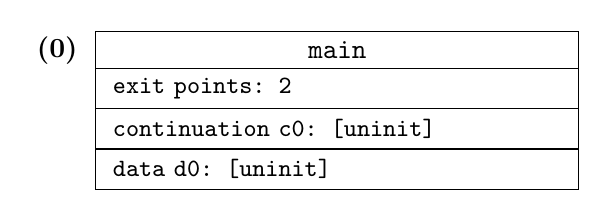
\begin{tikzpicture}
\node[font=\ttfamily] (main title) {main};
\node[row, below=0pt of main title] (main exit) {exit points: 2};
\node[row, below=0pt of main exit] (main c0) {continuation c0: [uninit]};
\node[row, below=0pt of main c0] (main d0) {data d0: [uninit]};
\node[draw, inner sep=0pt, fit=(main title) (main d0)] (main box) {};
\node[font=\bf, anchor=east] at ([xshift=-1mm, yshift=-2.5mm]main box.north west) {(0)};
\end{tikzpicture}
\end{center}

In step \textbf{(1)}, \texttt{initContinuation(c0, rhs, d0)} is executed. This instruction initializes $c_0$, setting its return address to the block \texttt{rhs}, its writing location to $d_0$, and its remote continuation reference to itself. This self link is necessary, as the other endpoint of the session, on the right-hand-side of the $\cutp$ in the source program, is within the same environment and uses the same continuation $c_0$.

\begin{center}
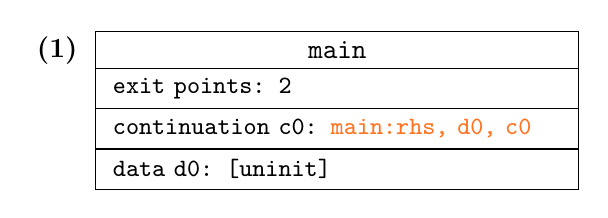
\begin{tikzpicture}
\node[font=\ttfamily] (main title) {main};
\node[row, below=0pt of main title] (main exit) {exit points: 2};
\node[row, below=0pt of main exit] (main c0) {continuation c0: \changed{main:rhs, d0, c0}};
\node[row, below=0pt of main c0] (main d0) {data d0: [uninit]};
\node[draw, inner sep=0pt, fit=(main title) (main d0)] (main box) {};
\node[font=\bf, anchor=east] at ([xshift=-1mm, yshift=-2.5mm]main box.north west) {(1)};
\end{tikzpicture}
\end{center}

In step \textbf{(2)}, \texttt{callProcess(foo, exit point, c1 <- c0)} is executed, moving the program counter to the \texttt{entry} block of \texttt{foo}, and creating a new environment for \texttt{foo}. Since $c_0$ was passed as an argument, it is copied to $c_2$ in \texttt{foo}. The continuation referenced by $c_0$, which is $c_0$ itself, is linked to $c_1$. Both environments now hold opposite endpoints of the same session $x$, represented by $c_0$ and $c_1$, which are linked to each other. The writing location of $c_0$ is changed to $d_2$, allowing data written by \texttt{main} to be read by \texttt{foo}. Finally, since the instruction is marked as an exit point, the remaining exit point count of \texttt{main} is decremented.

\begin{center}
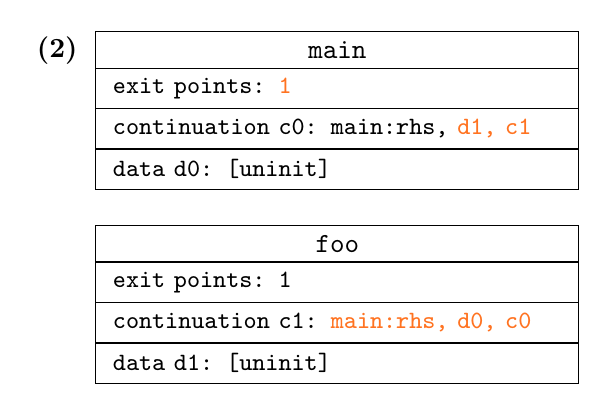
\begin{tikzpicture}
\node[font=\ttfamily] (main title) {main};
\node[row, below=0pt of main title] (main exit) {exit points: \changed{1}};
\node[row, below=0pt of main exit] (main c0) {continuation c0: main:rhs, \changed{d1, c1}};
\node[row, below=0pt of main c0] (main d0) {data d0: [uninit]};
\node[draw, inner sep=0pt, fit=(main title) (main d0)] (main box) {};
\node[font=\ttfamily, below=2cm of main title.south] (foo title) {foo};
\node[row, below=0pt of foo title] (foo exit) {exit points: 1};
\node[row, below=0pt of foo exit] (foo c1) {continuation c1: \changed{main:rhs, d0, c0}};
\node[row, below=0pt of foo c1] (foo d1) {data d1: [uninit]};
\node[draw, inner sep=0pt, fit=(foo title) (foo d1)] (foo box) {};
\node[font=\bf, anchor=east] at ([xshift=-1mm, yshift=-2.5mm]main box.north west) {(2)};
\end{tikzpicture}
\end{center}

In step \textbf{(3)}, \texttt{writeExpression(c1, 17)} is executed, which writes the integer $17$ to the writing location of $c_1$, which is $d_0$.

In step \textbf{(4)}, \texttt{continue(c1, ret)} is executed, passing control back to the return address stored in $c_1$, which is the \texttt{rhs} block in \texttt{main}. The continuation referenced by $c_1$, $c_0$, has its return address set to \texttt{ret} in \texttt{foo}, allowing control to return to \texttt{foo} later on.

\begin{center}
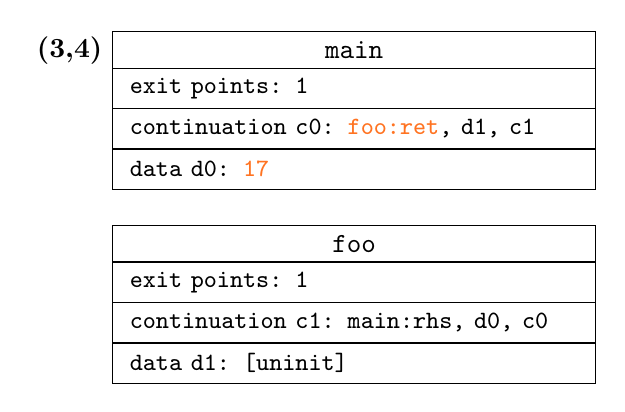
\begin{tikzpicture}
\node[font=\ttfamily] (main title) {main};
\node[row, below=0pt of main title] (main exit) {exit points: 1};
\node[row, below=0pt of main exit] (main c0) {continuation c0: \changed{foo:ret}, d1, c1};
\node[row, below=0pt of main c0] (main d0) {data d0: \changed{17}};
\node[draw, inner sep=0pt, fit=(main title) (main d0)] (main box) {};
\node[font=\ttfamily, below=2cm of main title.south] (foo title) {foo};
\node[row, below=0pt of foo title] (foo exit) {exit points: 1};
\node[row, below=0pt of foo exit] (foo c1) {continuation c1: main:rhs, d0, c0};
\node[row, below=0pt of foo c1] (foo d1) {data d1: [uninit]};
\node[draw, inner sep=0pt, fit=(foo title) (foo d1)] (foo box) {};
\node[font=\bf, anchor=east] at ([xshift=0mm, yshift=-2.5mm]main box.north west) {(3,4)};
\end{tikzpicture}
\end{center}

In step \textbf{(5)}, \texttt{writeExpression(c0, "Res:\ " + move(d0, int))} is executed. This instruction reads the integer $17$ from $d_0$, constructs the string \texttt{"Res:\ 17"}, and writes it to the writing location of $c_0$, which is $d_1$.

In step \textbf{(6)}, \texttt{finish(c0, exit point)} is executed, causing a jump to the code address stored in $c_0$, which is the \texttt{ret} block of \texttt{foo}. Both $c_0$ and the continuation it references, $c_1$, are considered uninitialized and will not be used again. The exit point count of \texttt{main} is decremented, as before, reaching $0$. This signals that \texttt{main}'s environment will not be used again, and thus, can be destroyed.

\begin{center}
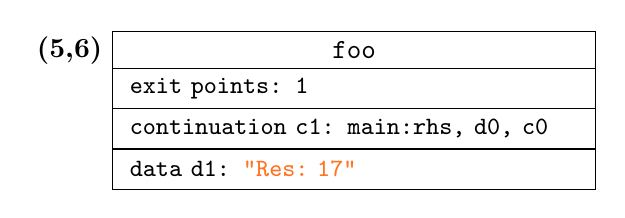
\begin{tikzpicture}
\node[font=\ttfamily] (foo title) {foo};
\node[row, below=0pt of foo title] (foo exit) {exit points: 1};
\node[row, below=0pt of foo exit] (foo c1) {continuation c1: main:rhs, d0, c0};
\node[row, below=0pt of foo c1] (foo d1) {data d1: \changed{"Res:\ 17"}};
\node[draw, inner sep=0pt, fit=(foo title) (foo d1)] (foo box) {};
\node[font=\bf, anchor=east] at ([xshift=0mm, yshift=-2.5mm]foo box.north west) {(5,6)};
\end{tikzpicture}
\end{center}

In step \textbf{(7)}, \texttt{printLine(move(d1, string))} is executed, printing the string \texttt{"Res:\ 17"} to the standard output.

Finally, in \textbf{(8)}, \texttt{popTask(exit point)} is executed, terminating the program. Since the exit point count is $1$, and the instruction is an exit point, the environment is destroyed, avoiding memory leaks.

\begin{center}
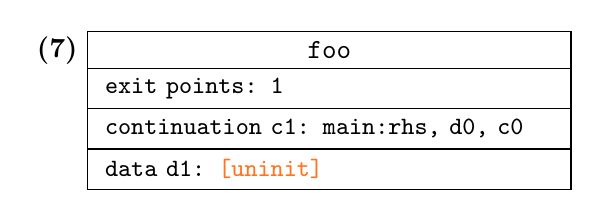
\begin{tikzpicture}
\node[font=\ttfamily] (foo title) {foo};
\node[row, below=0pt of foo title] (foo exit) {exit points: 1};
\node[row, below=0pt of foo exit] (foo c1) {continuation c1: main:rhs, d0, c0};
\node[row, below=0pt of foo c1] (foo d1) {data d1: \changed{[uninit]}};
\node[draw, inner sep=0pt, fit=(foo title) (foo d1)] (foo box) {};
\node[font=\bf, anchor=east] at ([xshift=0mm, yshift=-2.5mm]foo box.north west) {(7)};
\end{tikzpicture}
\end{center}

\subsubsection{Data Representation} \label{subsubsection:IRSlots}

\ac{IR} programs are completely platform agnostic, and thus, data types and addresses are described through their composition of \textit{slots}, instead of concrete byte sizes and offsets. A slot $S$ is a unit of data in the \ac{IR}, and is defined as
\[\begin{aligned}
S ::= &\ \ints \mid \bools \mid \strings \mid \tags \mid \conts\\\mid&\ \cells{T} \mid \exponentials \mid \types \mid \vars{i}\end{aligned}\]
where $\ints$, $\bools$ and $\strings$ represent the basic data types, $\tags$ represents a \ac{CLASS} choice, $\conts$ a continuation reference, $\cells{T}$ a reference to a shared state cell with contents described by the slot tree $T$ (introduced below), $\exponentials$ an exponential reference, $\types$ a stored type parameter, and $\vars{i}$ a type parameter declared in the current process header. 

In order to model branching data types (such as choices from \ac{CLASS}), data layouts are described through trees of slots, instead of plain sequences. A slot tree $T$ is defined recursively as
\[
T ::= \nilst \mid \seqst{S_1; \dots; S_n; T} \mid \tagst{T_1 \tagsepst \dots \tagsepst T_n}
\]
where $\nilst$ is the empty slot tree, $\seqst{S_1; \dots; S_n; T}$ is a sequence of a slots $S_1; \dots; S_n$ followed by a slot tree $T$, and $\tagst{T_1 \tagsepst \dots \tagsepst T_n}$ is a $\tags$ slot followed by a choice between the slot trees $T_1$ to $T_n$. For example, $\seqst{\ints; \tagst{\seqst{\bools} \tagsepst \seqst{\strings}}}$ describes an integer followed by a tag, which, if $0$, is followed by a boolean, or if $1$, by a string.

Data sections are described within process headers by a sum of slot trees describing the possible layouts of data that can be stored on them. For example, $\texttt{data d0:}\ \combst{\seqst{\ints} + \seqst{\strings}}$ describes a data section $d_0$ which can either store an $\ints$ or a $\strings$.

Data is addressed through \textit{data location}, denoted as $\dataol{b}{o}$, where $b$ is a base address and $o$ an offset. A base address may be, for example, a data section (e.g., $d_0$), or  writing   location given by a continuation (e.g., $c_0$). An offset is defined by two slot trees, written as $\offs{P}{F}$, $P$ describing the data being skipped (named \textit{past}), and $F$ describing the data that may come next (named \textit{future}). The future tree is necessary to determine the alignment of the data being accessed. For example, the location $\datal{d_0}{\seqst{\ints}}{\seqst{\ints}}$ refers to the second integer stored in $d_0$, while the location $\datal{c_0}{\seqst{\bools}}{\seqst{\strings}}$ refers to a string stored in the writing location of the continuation $c_0$, after a boolean. When the offset is zero, it is omitted for brevity. For example, $d_0$ as a data location is equivalent to $\datal{d_0}{\nilst}{\nilst}$ or just $d_0.0$ - the future slot trees are unnecessary for empty past slot trees.

\subsection{Translating CLASS to the IR}

Compilation of \ac{CLASS} processes into \ac{IR} programs always occurs within the context of a single \ac{IR} process. As \ac{CLASS} processes are compiled into \ac{IR} instructions, new information is added to the \ac{IR} process header, along with the new instructions and blocks. Changes to the header of the \ac{IR} process are denoted by
\begin{center}
\setlength{\abovedisplayskip}{-4pt}
\begin{minipage}{0.3\linewidth}\begin{equation}\makecont{c}\label{eq:makecont}\end{equation}\end{minipage}
\hfill
\begin{minipage}{0.3\linewidth}\begin{equation}\makedata{d}{T}\label{eq:makedata}\end{equation}\end{minipage}
\hfill
\begin{minipage}{0.3\linewidth}\begin{equation}\makeblock{l}\label{eq:makeblock}\end{equation}\end{minipage}
\end{center}
Action \Cref{eq:makecont} adds a new continuation to the process header, identified by $c$. Action \Cref{eq:makedata} creates a new data section with data layout $T$ identified by $d$. Action \Cref{eq:makeblock} generates a unique label $l$ for a new instruction block within the process body.

\subsubsection{Compilation State}

The compiler must keep track of information regarding the type parameters and the state of each session endpoint within the process being compiled. This state is referred to as the environment, and is represented by a tuple $(\theta, \Delta)$, where $\theta$ is the type environment and $\Delta$ is the session environment.

A type environment $\theta$ is a mapping from type variables to a tuple $(p, t)$ where $p$ is the polarity of the type variable ($+$ or $-$) and $t$ is its identifier (e.g, $t_0$, $t_1$) within the header of the process being compiled. $\polarityof{\theta}{X}$ and $\typeidof{\theta}{X}$ are defined as the polarity and identifier of type variable $X$ in the type environment $\theta$, respectively. A type with positive polarity is one for which sessions of that type are used to write data, while a type with negative polarity is one for which sessions of that type are used to read data.

The function $\polarityof{\theta}{A}$ is further extended to all session types $A$ through pattern matching. For example, \[\polarityof{\theta}{\colintt} = - \quad\text{and}\quad \polarityof{\theta}{\bangt{A}} = +\]

A session environment $\Delta$ is a mapping from session endpoint names to session states. Each session state is a tuple $(c, d, o)$, where $c$ is the continuation identifier associated with the session endpoint (or $0$ if there's no continuation), $d$ is the identifier of the data section from which data is read (or $0$ if there's no data section), and $o$ is the data offset to apply to the location of the next write or read operation on the session.

Given a session environment $\Delta$, $\Delta[x \mapsto (c, d, o)]$ is defined as the updated mapping where session endpoint $x$ is mapped to the new session state $(c, d, o)$. Additionally $\continuationof{\Delta}{x}$, $\localdataof{\Delta}{x}$ and $\offsetof{\Delta}{x}$ are defined as the continuation, data section and data offset associated with session $x$ in the session environment $\Delta$, respectively.

For convenience, $\readlocof{\Delta}{x}$ and $\writelocof{\Delta}{x}$ are denoted as the current data location from which data of session endpoint $x$ is to be read, and the data location into which data for session $x$ is to be written, respectively. Both take into account the offset, and are defined as \[\readlocof{\Delta}{x} = \dataol{\localdataof{\Delta}{x}}{\offsetof{\Delta}{x}} \hspace{5em} \writelocof{\Delta}{x} = \dataol{\continuationof{\Delta}{x}}{\offsetof{\Delta}{x}}\]

\paragraph{Advacing Offsets}

When more than one slot is read from or written to a session endpoint in succession, the session's offset must be advanced accordingly. To this end, the concatenation of offsets must be defined. Given two offsets $o_1 = \offs{P_1}{F_1}$ and $o_2 = \offs{P_2}{F_2}$, their concatenation is defined as $\concatst{o_1}{o_2} = \offs{(\concatst{P_1}{P_2})}{F_2}$, where $\concatst{P_1}{P_2}$ is the concatenation of the two slot trees. In other words, when two offsets are concatenated, the resulting offset has concatenates both past slot trees, and keeps the future slot tree of the second offset. Slot tree concatenation is defined as replacing every leaf of the first slot tree with the second tree.

To simplify the translation definitions, $\advancech{\Delta}{x}{p}{\theta}{S}{A}$ is denoted as the session environment $\Delta$ where the offset of session $x$ is either reset, or advanced by the necessary offset to skip over the slots $S$. The decision is made based on whether the polarity $p$ (either $+$ or $-$) matches the polarity of the type $A$ in the type environment $\theta$. If they match, the new offset is computed as $\concatst{\offsetof{\Delta}{x}}{(\slotoffset{S}{\slots{\theta}{A}})}$, where $S$ is a slot tree describing the data which was just read or written, and $\slots{\theta}{A}$ is the slot tree corresponding to type $A$, which will be defined below. Otherwise the new offset is $0$. Formally, $\advancech{\Delta}{x}{p}{\theta}{S}{A}$ is defined as
\[\begin{cases}
    \Delta[x \mapsto (\continuationof{\Delta}{x}, \localdataof{\Delta}{x}, \concatst{\offsetof{\Delta}{x}}{(\slotoffset{S}{\slots{\theta}{A}})})] & \text{if } p = \polarityof{\theta}{A} \\
    \Delta[x \mapsto (\continuationof{\Delta}{x}, \localdataof{\Delta}{x}, 0)] & \text{otherwise}
\end{cases}\]

\subsubsection{Mapping Session Types to Slot Trees} \label{subsubsection:MappingSessionTypesToSlots}

Since \ac{IR} data types are represented through slot trees, a mapping from session types to slot trees is necessary. This mapping is denoted by $\slots{\theta}{A}$, where $\theta$ is the type environment and $A$ is the session type being mapped. The full definition of the mapping is omitted for brevity. The mapping is defined first for strictly positive session types. For example,
\[\begin{aligned}&\slots{\theta}{\closet} = \nilst
  &&\slots{\theta}{\lintt} = \seqst{\ints} \\ &\slots{\theta}{\sendt{A}{B}} = \seqst{\conts; \slots{\theta}{B}} &&\slots{\theta}{X} = \seqst{\typeidof{\theta}{X}}\\
\end{aligned}\]

To extend this concept to all session types, we must consider that session types may have multiple segments of data exchange, separated by changes in polarity. We can separate a session type into its segments by replacing every continuation of a different polarity with the unit type of that polarity ($\closet$ or $\waitt$) on the current segment and starting a new segment with the continuation. 

For example, $\sendt{\lintt}{\recvt{\lstringt}{\closet}}$ can be split into three segments: first $\sendt{\lintt}{\closet}$, then $\recvt{\lstringt}{\waitt}$ and finally  $\closet$. Each segment is either strictly positive or strictly negative. Strictly negative segments can be turned into strictly positive segments by computing their dual types. Thus, we can map each segment to a slot tree through the $\slots{\theta}{A}$ function defined above. The set of all slot trees corresponding to the segments of a session type $A$ is denoted by $\allslots{\theta}{A}$, and the set of slot trees corresponding to the negative segments by $\alllocalslots{\theta}{A}$. Sets of slot trees are termed \textit{layouts}, as they describe the full data exchanged over a session.

\subsubsection{Instruction Translation and Exit Point Counting}

The translation of \ac{CLASS} processes into \ac{IR} is defined through two main functions. The first, $\getinstructions{\theta}{\Delta}{P}$, translates a \ac{CLASS} process $P$ on an environment $(\theta, \Delta)$ into a sequence of \ac{IR} instructions. The second, $\getendpoints{\theta}{P}$, counts the number of exit points in a process $P$ on a type environment $\theta$. Both functions are defined recursively through pattern matching on processes.

The translated code implements the write-to-read adjustment of the \ac{SAM} through the placement of \texttt{continue} instructions whenever the polarity of a session changes from positive to negative. To simplify the definition of the translation rules, a pseudo-instruction $\texttt{continueIfNegative}(\theta, \Delta, x, A)$ is defined as
\[\begin{cases}
    \begin{array}{l}
        \quad\textcolor{forestgreen}{\texttt{\% }\makeblock{\texttt{label}}} \\
        \quad\texttt{continue}(\continuationof{\Delta}{x}, \texttt{label}) \\
        \texttt{label:} \\
        \hline
    \end{array} & \text{ if } \polarityof{\theta}{A} = -\\
    \quad\ \ \textcolor{forestgreen}{\texttt{\%\ empty}} & \text{ otherwise}\\
\end{cases}\]
which means that if and only if $\polarityof{\theta}{A} = -$, $\texttt{continueIfNegative}$ is replaced by a \texttt{continue} instruction, and the next instructions are placed in a new block. Otherwise, \texttt{continueIfNegative} is simply removed from the instruction sequence.

\subsubsection{Translating Process Definitions} A \ac{CLASS} program is a set of process definitions, each with a unique name. For each process definition, a set of resulting \ac{IR} processes is generated, one for each possible combination of polarities of the process definition type parameters. This guarantees that the polarity of each type parameter is always known at compile time, which is important as it greatly affects the flow of control of the translated code.

For each resulting \ac{IR} process, an environment $(\theta, \Delta)$ is initialized. The type environment $\theta$ maps each type parameter name to its polarity and unique identifier within the process header. The session environment $\Delta$ maps each linear and exponential argument of the process definition to their initial session state.

The body of the \ac{IR} process is built from the process definition's body $P$ by calling the instruction translation function $\getinstructions{\theta}{\Delta}{P}$. The number of exit points of the \ac{IR} process is set to $\getendpoints{\theta}{P}$.

\subsubsection{Translating Process Constructs}

The compilation definitions for the $\cutc{P}{x:A}{Q}$ process on an environment $(\theta, \Delta)$ are shown below. It is assumed, without loss of generality, that $\polarityof{\theta}{A} = +$, and thus, that $P$ will be writing to $x$ before $Q$ executes - if $A$ were negative, $P$ and $Q$ could simply be swapped. The layout $\allslots{\theta}{A}$ is given to $d$, guaranteeing that enough space is allocated for all data received by both endpoints of $x$.
\begin{compilation}{\theta}{\Delta}{\cutc{P}{x: A}{Q}}
{\getendpoints{\theta}{P} + \getendpoints{\theta}{Q}}
    \commentline{\makecont{c}, \makeblock{\texttt{rhs}}, \makedata{d}{\allslots{\theta}{A}}}
    \initcontinuation{c}{\texttt{rhs}}{d}
    \recurse{\theta}{\Delta[x \mapsto (c, d, 0)]}{P}
    \labelir{rhs}
    \recurse{\theta}{\Delta[x \mapsto (c, d, 0)]}{Q}
\end{compilation}

The instructions initialize a new continuation $c$ with a new block $\makeblock{\texttt{rhs}}$ as the return address and a new data section $d$ as a writing location. Both $P$ and $Q$ are recursively translated on a new environment where $x$ is bound to $(c, d, 0)$. $P$ is placed on the original block, and $Q$ placed on the new block \texttt{rhs}. The number of exit points of the instructions is the sum of the number of exit points of both $P$ and $Q$. 

The $\closec{x}$ process indicates that a session $x$ is finished. As on \ac{SAM}, control is passed to the other endpoint of $x$, never returning back. This jump is performed with the \texttt{finish} instruction, taking as argument the continuation of session $x$, obtained from $\Delta$.
\begin{compilation}{\theta}{\Delta}{\closec{x}}{1}
    \finishcont{\continuationof{\Delta}{x}}{\hasexitpoint}
\end{compilation}

The $\waitc{x}{P}$ process is skipped and simply compiled directly as $P$: $\getendpoints{\theta}{\waitc{x}{P}} \equiv \getendpoints{\theta}{P}$, $\getinstructions{\theta}{\Delta}{\waitc{x}{P}} \equiv \getinstructions{\theta}{\Delta}{P}$. No instructions are generated for the wait action, as the action of waiting for the other side of the channel is already performed implicitly by the \ac{SAM} execution scheme.

The $\sendc{x}{y}{P}Q$ process creates a new session $y$, sending one of its endpoints over session $x$. The other endpoint of $y$ is then used in process $P$, while process $Q$ continues using session $x$. To model this behavior, the continuation $c$ and and data section $d$ are created to implement session $y$, where $A$ is the type of session $y$. The layout $\alllocalslots{\theta}{A}$ is given to $d$, guaranteeing that enough space is allocated for all data received by the local endpoint of $y$.

\begin{compilation}{\theta}{\Delta}{\sendc{x}{y}{P}{Q}}
{\getendpoints{\theta}{P} + \getendpoints{\theta}{Q}}
    \commentline{\makecont{c}, \makeblock{\texttt{lhs}}, \makedata{d}{\alllocalslots{\theta}{A}}}
    \initcontinuation{c}{\texttt{lhs}}{d}
    \writecontinuation{\writelocof{\Delta}{x}}{c}
    \continueifneg{\theta}{\Delta}{x}{A} \comment{\text{where } x:A \text{ in }Q}
    \recurse{\theta}{\advancech{\Delta}{x}{+}{\theta}{\seqst{\conts}}{A}}{Q}
    \labelir{lhs}
    \recurse{\theta}{\Delta[y \mapsto (c, d, 0)]}{P}
\end{compilation}

The continuation $c$ is initialized with a return address pointing to \texttt{lhs} and $d$ as a writing location. The continuation $c$ is then written to the writing location of session $x$, $\writelocof{\Delta}{x}$. As before, a write-to-read adjustment might be necessary, and thus, the \texttt{continueIfNegative} pseudo-instruction is used.

The $\recvc{x}{y}P$ process receives a session endpoint $y$ over session $x$, which then is used in process $P$. As on the \ac{SAM}, control must be passed to the other side of session endpoint $y$ if its type is negative, ensuring that the writing side of the session executes first. To receive data through $y$, a data section $d$ is created. A continuation $c$ is also created to bind $y$ to.
\begin{compilation}{\theta}{\Delta}{\recvc{x}{y: A}{P}}
{\getendpoints{\theta}{P}}
    \commentline{\makecont{c}, \makedata{d}{\alllocalslots{\theta}{A}}}
    \bindcontinuation{c}{\readlocof{\Delta}{x}}{d} 
    \continueifneg{\theta}{\Delta}{y}{A}
    \recurse{\theta}{\advancech{\Delta}{x}{-}{\theta}{\seqst{\conts}}{B}[y \mapsto (c, d, 0)]}{P} \comment{x:B \text{ in }P}
\end{compilation}

\subsection{Translating the IR to C}

The last phase of the compilation pipeline is the translation from the \ac{IR} to C. This phase takes as input the \ac{IR} produced by the compilation scheme described in the previous section, and produces a C program which implements the semantics of the \ac{IR}. This C program can then be compiled with \ac{GCC} to produce an executable which runs a computation equivalent to the original \ac{CLASS} program. The translated code depends only on the standard C library and on \texttt{pthread}, if concurrency is enabled. Additionally, it makes extensive use of the \ac{GCC} extension for computed gotos, used to efficiently implement continuations.

\subsubsection{Slot Memory Layouts}

In the \ac{IR} abstract machine, the concept of data is abstracted away into slots. When translating \ac{IR} programs to C code, these slots must be translated to concrete, byte-addressed, memory layouts. To this end, a memory layout is defined as a tuple $L = (s, a)$, where $s$ is the size in bytes of the layout, and $a$ is the alignment in bytes the layout must have in memory. Both $s$ and $a$ are not constants, but C expressions which can be evaluated at runtime. This is necessary due to type parameters having layouts known only at runtime.

The memory layout of a slot $S$ on a given target architecture $\arch$ is denoted as $\slotlayout{\sigma}{S}$, where $\sigma$ is a map between type parameters and their layouts. A target architecture $\arch$ is a mapping from C types to their memory layouts, such that $\archlayout{type} = (s, a)$ where $s$ and $a$ where, respectively, the size and alignment of \texttt{type} on the target architecture. For example,
\[\slotlayout{\sigma}{\ints} = \archlayout{\texttt{int}} \quad\quad \slotlayout{\sigma}{\vars{i}} = \sigma(t_i)\]

The definition of $\slotlayout{\sigma}{s}$ is extended to support both slot trees, and sets of slot trees. The layout of a slot tree is defined as the concatenation of the layouts of each of its slots, and maximum across any branches, while the layout of a set of slot trees is defined as the maximum layout among all its trees.

\subsubsection{Environment Memory Layout}

\ac{IR} environments store all state related to a process invocation. In the translated C programs, environments are represented as heap allocated byte buffers. The environment layout $\envlayout$ specifies at compile time how environment buffers will be indexed at runtime.

An environment layout $\envlayout$ is a compile-time data structure which describes the byte offsets at which each entry of the environment can be found. This layout is computed from the header of the \ac{IR} process being compiled. It is obtained trivially by concatenating the layouts of each of its continuations, data sections and other entries, in the order they appear in the process header. Data section layouts, for example, depends on the type of the data they store. This layout is computed from $\slotlayout{\sigma}{S}$, where $S$ is the set of slot trees of the data section, and $\sigma(t_i) = \texttt{access}(\envlayouttype{\texttt{env}}{t_i})$ is a mapping between type parameters and their layouts, fetched from the environment itself, pointed to by \texttt{env}.

\subsubsection{Execution and Registers}

The \ac{IR} has no concept whatsoever of stacks or function calls, and processes cannot be mapped to C functions efficiently due to their use of continuations. Thus, the entire \ac{IR} abstract machine is implemented within a single C function named \texttt{executor}. \ac{IR} blocks are translated to C labels within this function, and \ac{IR} instructions are translated to C statements. Jumps between instructions such as \texttt{callProcess} and \texttt{continue} are implemented through gotos to the corresponding C labels, or to their addresses stored in continuations.

Register variables declared within the \texttt{executor} function are used to store the current state, such as a pointer to the current environment, and also temporary values for instruction execution.

Each thread of execution runs the \texttt{executor} function, which takes as argument information about the initial code address to execute on. The main thread of the program sets this code address to the entry block of the \texttt{main} process, allocating a new environment for it, while new threads are spawned into existing environments.

\section{Optimization Techniques} \label{sec:optimizations}

\subsection{Leveraging Type Properties}

The compiler presented in the previous section does not take any advantage of the fact that many types in the language can be handled more efficiently than the general case. For example, the type $\sendt{\lintt}{\lintt}$ is stored as a reference to a continuation (essentially a closure) followed by an integer. The closure producing the $\lintt$ will eventually be executed, producing a single integer and immediately terminating. Instead of sending this continuation, the integer could be computed immediately and sent directly, avoiding pointer indirection and unnecessary jumps, saving memory and time.

Types are thus optimized based on their properties. In the example above, the optimization is possible because $\lintt$ is a \textit{value type}, i.e., strictly positive. Sends of positive value types can always be optimized this way, as the execution of a session of a positive value type always produces the value   immediately, and then terminates.

This concept can also be extended to other domains of the language, such as exponentials. If a cloning operation can be defined for a value type, as is the case for integers and booleans, for example, then an exponential session of that type can be optimized to store the value directly. This effectively turns most exponential closures, which recompute their value every time they're used, into much more efficient value copies. 

\subsection{Optimizing Single Exit Points and Tail Calls}

In the base version of the compiler, every exit point instruction decrements the exit point counter of the current environment, and if it reaches zero, the environment is destroyed. For processes with a single exit point, this is wasteful --- there is no need to maintain an exit point counter. The C code generation phase takes advantage of this, omitting exit point handling code when the \ac{IR} process has a single exit point, avoiding unnecessary accesses and branches.

Tail calls, i.e., recursive process calls executed when a single exit point is left, are optimized to reuse the current process environment instead of allocating a new one, avoiding the overhead of memory allocation and deallocation, and greatly improving performance.

\subsection{Simplifying IR Programs}

The previously mentioned transformations introduce many optimization opportunities in the generated \ac{IR} code itself. For example, below is the result of compiling a send of positive value type. A new continuation $c_2$ is introduced only for writing to $c_1$. In this case, it could be replaced entirely by direct writes to $c_1$.

\begin{lstlisting}[language=IR, frame=bottom]
    initContinuation(c2, send_rhs_2, c1)
    writeExpression(c2, 1)
    finish(c2, exit point)
send_rhs_2:
    ... // send rhs
\end{lstlisting}

A symbolic execution on each \ac{IR} process is performed, extracting information about the control flow and known state of the process environment at each instruction. This information is then used to remove unnecessary instructions and merging \ac{IR} blocks when possible. The code above is reduced to \texttt{writeExpression(c1, 1)}.

Another useful result from the symbolic execution is getting information on which exit point instructions are guaranteed to not be the last instruction executed by the process. In these cases, the exit point marking can be removed, as the process will never terminate at that point, saving unnecessary checks.

\section{Results}

\subsection{Correctness}

The described compilation scheme, along with all described optimizations, was fully implemented in Java, within the existing \ac{CLASS} and \ac{SAM} interpreters code base \citep{Rocha:2021:artifact,Caires:2024:artifact}.

A comprehensive suite of more than 180 unit tests written in the \ac{CLASS} language was developed. This suite covers all features of the language, including edge cases relevant to the implemented optimizations. Each test is composed of a \ac{CLASS} source file, and optionally, a number of input and expected output files. This suite was run with \texttt{valgrind} and multiple \texttt{gcc} sanitizers enabled to further validate the absence of memory errors data races.

Multiple complex \ac{CLASS} programs were compiled, tested and integrated into the test suite in order to further validate the correctness of the generated code when many features are combined. These programs include an implementation of the Game of Life cellular automaton \citep{GameOfLife:1970}, a prime sieve, a linked list implementation, a simulation of the dining philosophers problem, and other programs making extensive use of both shared state, polymorphism, recursion and exponentials.

\subsection{Benchmarks}

After the entirety of \ac{CLASS} was supported by the compiler, and extensive testing was performed to validate the correctness of the generated code, focus was shifted to measuring and improving the performance of the generated code. To this end, benchmarking \ac{CLASS} programs were developed along with equivalent Haskell implementations. Many compiler configurations were benchmarked, including the interpreted execution of the same program using both the \ac{CLASS} and \ac{SAM} interpreters, and the equivalent Haskell implementations, compiled with GHC \texttt{-O2}. All presented results are averaged over 10 runs, and were obtained on a machine with an Intel Core i9-12900K CPU and 32GB of RAM, running NixOS 25.05.

\begin{figure}
    \centering
    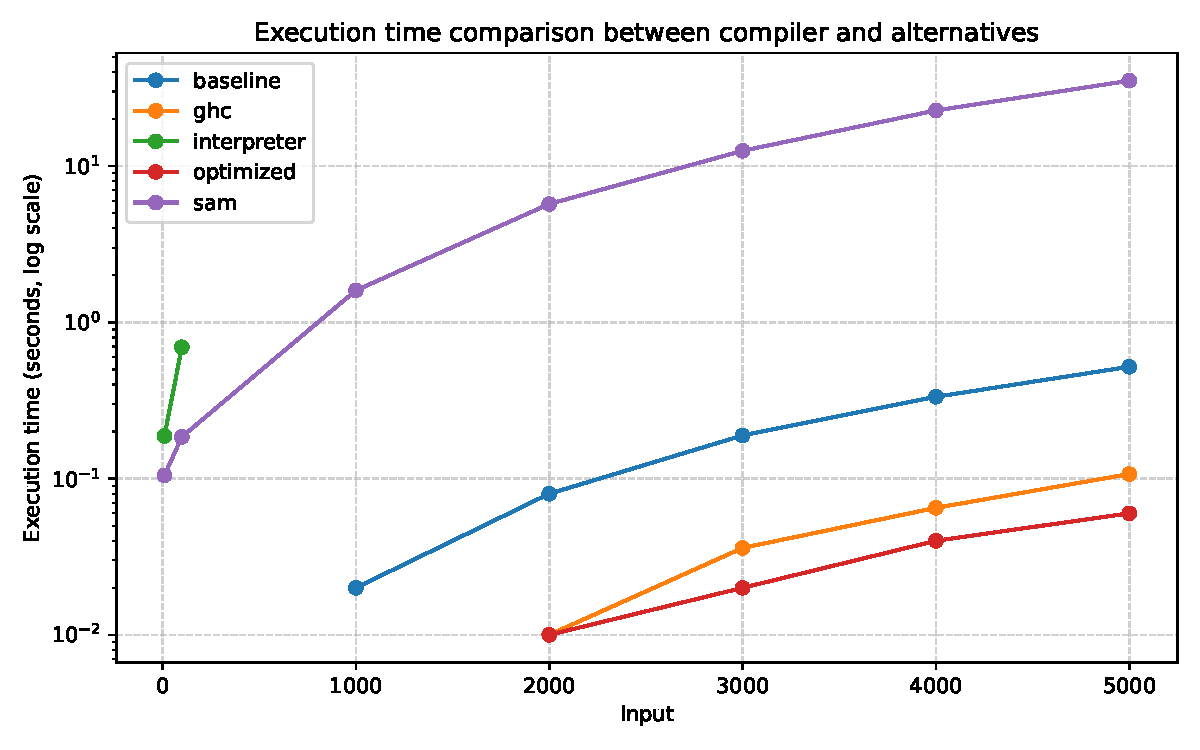
\includegraphics[width=0.8\linewidth]{./Images/execution_time_sieve_compiler_vs_alternatives.pdf}
    \caption{Prime sieve parametrized by prime count.}
    \label{fig:SieveBenchmarkCompilerVsAlternatives}
    \Description{Prime sieve parametrized by prime count.}
\end{figure}

\begin{figure}
    \centering
    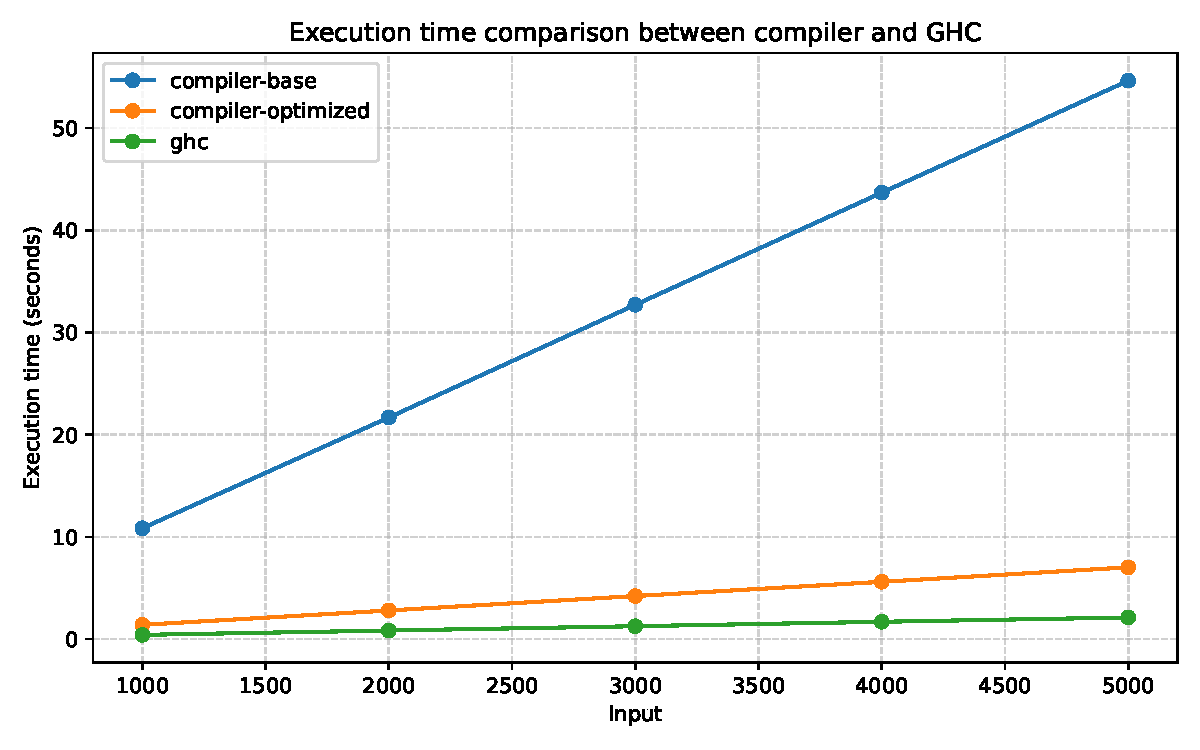
\includegraphics[width=0.8\linewidth]{./Images/execution_time_gol_compiler_vs_ghc.pdf}
    \caption{Game of Life parametrized by generation count.}
    \Description{Game of Life parametrized by generation count.}
    \label{fig:GOLBenchmarkCompilerVsGHC}
\end{figure}

The first benchmark program computes prime sieve numbers using the Turner's Sieve algorithm, generating a list of prime numbers up to a given count, taken as input. This benchmark was chosen because it is a simple yet computationally intensive program. On \Cref{fig:SieveBenchmarkCompilerVsAlternatives}, the execution time and the maximum \ac{RSS}, representing the peak memory usage, are compared between the original \ac{CLASS} interpreter, the \ac{SAM} interpreter, the unoptimized (baseline) compiler, the fully optimized compiler, and the equivalent Haskell implementation. The original interpreter cannot handle more than 150 primes due to operating system limits on the number of threads. The results show that the fully optimized compiler achieves a speed up of more than 100x compared to the \ac{SAM} interpreter, a speedup of more than 5x compared to the unoptimized compiler, and also that it outperforms GHC.

The second benchmark program implements a functional version of the Game of Life cellular automaton \citep{GameOfLife:1970}. All runs were given the same 17x17 initial configuration containing the \textit{Kok's Galaxy}\footnote{\url{https://conwaylife.com/wiki/Kok\%27s_galaxy}, accessed 2025-10-04} pattern, and were parametrized by the number of generations to compute. In this benchmark, shown in \Cref{fig:GOLBenchmarkCompilerVsGHC}, the optimized compiler performs slower than the Haskell implementation, by a factor of approximately 2.5x. We suspect that with further optimizations, such as allocating data in registers and reusing sessions and data sections, the Haskell implementation can be surpassed.

A third benchmark, covering the shared state features of \ac{CLASS}, was also developed, but is not presented here due to space constraints. On each benchmark, the performance of multiple compiler configurations was also evaluated, covering different combinations of the optimizations presented in \Cref{sec:optimizations}. The results are shown in detail in the full thesis document.

\section{Conclusion and Future Work}

\subsection{Conclusions}

In this thesis, a novel solution for compiling a linear session-typed language, \ac{CLASS} \cite{Rocha:2023}, into efficient C code was designed and implemented. The solution preserves the semantics and safety guarantees of the source language, while generating code that is orders of magnitude faster than the interpreted execution of \ac{CLASS} programs. The compilation scheme is based on the sequential execution model of \ac{CLASS} used by the \acf{SAM} \cite{Caires:2024}.

The developed solution consists of a type-directed compilation algorithm which translates \ac{CLASS} programs into an \acf{IR}, on which several optimizations are performed, before finally being translated into C code. The compilation makes use of the information available in the session types of \ac{CLASS} to generate efficient code, avoiding unnecessary runtime checks and garbage collection.

All program data, excluding exponential closures and shared state cells, is stored in structures associated to processes, similar to the stack frames used in imperative languages, but where the frames are organized into a spaghetti stack. Instead of the traditional single return address, each frame stores a continuation for each unfinished session in the process.

Communication over channels is compiled into direct memory writes into and reads from these frames, with sizes and offsets determined at compile time, excluding polymorphic code sections. When a sequence of writes on a given session finishes, control is passed back to the continuation stored in the active frame, following the execution model of the \ac{SAM}.

An implementation of the developed scheme was created, covering all of the features of \ac{CLASS}, including polymorphism, recursion and exponentials. The implementation, available on GitHub\footnote{\url{https://github.com/RiscadoA/class}}, was built in Java, on top of the existing \ac{SAM} codebase. A suite of tests was created to validate the correctness of the implementation, and the performance of the generated code was evaluated through a series of benchmarks, across different configurations. The compiler was shown to generate programs competitive with equivalent Haskell GHC compiled programs, being able to surpass them in some cases.

% #############################################################################
\subsection{Future Work}

The developed solution, while already showing promising results, still has several promising avenues for future improvements and optimizations. One such avenue is compiling to a lower level target language, such as LLVM IR, or assembly language. This could allow for, for example, storing frequently accessed data entirely in CPU registers, and committing them to memory only when absolutely necessary.

The \ac{IR} could also be optimized further, by removing, for example, redundant moves and copies of data, which are frequently generated by the current compilation scheme. Both sessions and local data sections could be reused if possible, reducing the memory footprint of the generated programs, and improving cache locality.

It would also be interesting to construct a formal proof of correctness for the compilation scheme, showing that the generated code preserves the semantics and safety of \ac{CLASS}. As the compiled code resembles the \ac{SAM} execution model, this proof could be based on its existing proof of correctness.

Concurrent channels have not been addressed in this work, as the focus was on generating efficient sequential code. The type system of the \ac{CLASS} language could be modified to distinguish between sequential and concurrent channels, allowing for the generation of efficient code for both channel types.

Finally, a standard library for \ac{CLASS} could also be developed, providing native implementations of common data structures such as arrays and maps, as currently these are emulated using recursive session types. This would greatly improve the usability and performance of \ac{CLASS} programs. This could be achieved by, for example, implementing a \ac{FFI} to C libraries.


%%
%% The next two lines define the bibliography style to be used, and
%% the bibliography file.
\bibliographystyle{ACM-Reference-Format}
\bibliography{extended-abstract}

\end{document}
\endinput
%%
%% End of file `extended-abstract.tex'.
